\documentclass[12pt, a4paper, parskip=full]{memoir} % for a short document
\usepackage[french,english]{babel}

\usepackage [vscale=0.76,includehead]{geometry}                % See geometry.pdf to learn the layout options. There are lots.
% \geometry{a4paper}                   % ... or a4paper or a5paper or ... 
% \geometry{landscape}                % Activate for for rotated page geometry
% \OnehalfSpacing
% \setSingleSpace{1.05}
% \usepackage[parfill]{parskip}    % Activate to begin paragraphs with an empty line rather than an indent


%===================================== packages
\usepackage{lipsum}
\usepackage{graphicx}
\usepackage{amsmath}
\usepackage{fullpage}
\usepackage{mathptmx} % font = times
\usepackage{helvet} % font sf = helvetica
\usepackage[latin1]{inputenc}
\usepackage{relsize}
\usepackage[T1]{fontenc}
\usepackage{tikz}
\usepackage{booktabs}
\usepackage{textcomp}%textquotesingle
\usepackage{multirow}
\usepackage{pgfplots}
\usepackage{url}
\usepackage{footnote}


%\usepackage{datetime2}
\usepackage[en-US,showdow=true]{datetime2}
\usepackage{amsmath}
\usepackage{graphicx}
\usepackage{wrapfig}
\usepackage{caption}
\usepackage{subcaption}
\usepackage{natbib}
\usepackage{hyperref}
\usepackage{datatool}
%============================================
\usetikzlibrary{arrows,shapes,positioning,shadows,trees}
\makesavenoteenv{tabular}
\makesavenoteenv{table}
%==============================================
\def\checkmark{\tikz\fill[scale=0.4](0,.35) -- (.25,0) -- (1,.7) -- (.25,.15) -- cycle;}
%Style des têtes de section, headings, chapitre
\headstyles{komalike}
\nouppercaseheads
\chapterstyle{dash}
\makeevenhead{headings}{\sffamily\thepage}{}{\sffamily\leftmark} 
\makeoddhead{headings}{\sffamily\rightmark}{}{\sffamily\thepage}
\makeoddfoot{plain}{}{}{} % Pages chapitre. 
\makeheadrule{headings}{\textwidth}{\normalrulethickness}
%\renewcommand{\leftmark}{\thechapter ---}
\renewcommand{\chaptername}{\relax}
\renewcommand{\chaptitlefont}{ \sffamily\bfseries \LARGE}
\renewcommand{\chapnumfont}{ \sffamily\bfseries \LARGE}
\setsecnumdepth{subsection}


% Title page formatting -- do not change!
\pretitle{\HUGE\sffamily \bfseries\begin{center}} 
\posttitle{\end{center}}
\preauthor{\LARGE  \sffamily \bfseries\begin{center}}
\postauthor{\par\end{center}}
\newcommand{\jury}[1]{% 
\gdef\juryB{#1}} 
\newcommand{\juryB}{} 
\newcommand{\session}[1]{% 
\gdef\sessionB{#1}} 
\newcommand{\sessionB}{} 
\newcommand{\option}[1]{% 
\gdef\optionB{#1}} 
\newcommand{\optionB} {}

\renewcommand{\maketitlehookd}{% 
\vfill{}  \large\par\noindent  
\begin{center}\juryB \bigskip\sessionB\end{center}
\vspace{-1.5cm}}
\renewcommand{\maketitlehooka}{% 
\vspace{-1.5cm}\noindent
\includegraphics[height=12ex]{pics/logo-uga.png}\hfill\raisebox{2ex}{
\includegraphics[height=14ex]{pics/logoINP.png}}\\
\bigskip
\begin{center} \large
Master of Science in Informatics at Grenoble \\
Master Informatique \\ 
Specialization \optionB  \end{center}\vfill}
% =======================End of title page formatting

\option{Graphics, Vision, and Robotics} 
\title{Sketch-Based Posing, Animation, and Interaction of Multiple Characters: Animating Dancing Couples} %\\\vspace{-1ex}\rule{10ex}{0.5pt} \\sub-title} 
\author{Sarah Anne Kushner}
\DTMlangsetup[en-US]{monthyearsep={\space}}
\newcommand{\mydate}{\DTMdisplaydate{2017}{06}{21}{2}}
\date{\mydate} % Delete this line to display the current date
\jury{
Research project performed at Inria Grenoble -- Rh\^one-Alpes\\\medskip
Under the supervision of:\\
Marie-Paule Cani and R\'emi Ronfard\\\medskip
Defended before a jury composed of:\\
James Crowley\\
Dominique Vaufreydaz\\
Jean-S\'ebastien Franco\\
Jo\"elle Thollot\\
}
\session{June \hfill 2017}
\setcounter{tocdepth}{4}
\setcounter{secnumdepth}{4}
 \maxsecnumdepth{subsubsection}
 

\setlength{\parindent}{0pt}
\nonzeroparskip 
 

%%% BEGIN DOCUMENT
\begin{document}
\selectlanguage{English} % french si rapport en français
\frontmatter
\begin{titlingpage}
\maketitle
\end{titlingpage}

%\small
%\setlength{\parskip}{-1pt plus 1pt}

\renewcommand{\abstracttextfont}{\normalfont}
\abstractintoc
\begin{abstract} 
Your abstract goes here... 
\end{abstract}
\abstractintoc

\renewcommand\abstractname{R\'esum\'e}
\begin{abstract} \selectlanguage{French}
Your abstract in French goes here... 
\end{abstract}
\selectlanguage{English}

\newpage

\renewcommand\abstractname{Acknowledgement}
\begin{abstract}
\newcommand{\ignore}[1]{}

\ignore{
I would like to officially say thank you to those without whom this thesis would not have been possible. It brings me joy to acknowledge the following people. \\

Thank you to\ignore{Associate Professor} David Breen,\ignore{Assistant Research Professor} Marcello Balduccini and\ignore{Associate Teaching Professor} Daryl Falco from Drexel University for being not only excellent and inspiring mentors and teachers, but also for helping and supporting me on my journey to study in France. \\

James Crowley deserves credit for making my move to France viable, and putting up with my numerous emails. I would also like to thank him for teaching me in the first semester of M2 along with all the other MoSIG M2 professors.\\

I would like to express my sincere gratitude to both my supervisers Marie-Paule Cani and R\'emi Ronfard for their invaluable assistance, guidance, and patience through the process of a Master thesis.\\

To the IMAGINE engineers Maguelonne de Brive and Julien Daval: thank you for answering my development questions and teaching me the mysterious ways of Blender. \\

I have so much appreciation for Tom. Thank you for letting me think out loud to you on the phone; comforting me when I freak out to you on the phone; sending me pictures of our baby bunny, Cinnamon Louise Bun; and providing me with constant encouragement all the way from the United States. \\

It wouldn't be fair not to mention and thank my dear dancer friends Ruth and Vivian for answering my sometimes obvious and weirdly specific questions about your experiences in dance and choreography.\\

Shout out to all the C1 bus drivers for getting me to and from Inria every day. Merci, au revoir. \\

Lastly, thank you to the jury for reading this report and listening to my presentation.
}

\end{abstract}



\cleardoublepage

\tableofcontents* % the asterisk means that the table of contents itself isn't put into the ToC
\normalsize

\mainmatter
\SingleSpace
%==============================CHAPTERS==================
\chapter{Introduction}
\lipsum[2-4]
\chapter{State-of-the-Art}\label{chap:sota}
\ignore{

\subsection{analyzing/classification}
Analysis of impression of robot bodily expression\\
Convolutional Pose Machines

\subsection{math/algorithms}
The Conjugate Residual Method for Constrained Minimization Problems -- 2015\\
Constrained Closed Loop Inverse Kinematics -- 2010
}



\section{Dance}
Sutton Dance Writing\\
Labanotation\\
Benesh Movement Notation

\section{Sketch-Based Systems}
The IMAGINE group at Inria has made it their mission to tackle this problem. They have made significant progress on a project where they aim to offer more intuitive tools to author 3D digital content. The IMAGINE team has invented (1) a type of notation made especially for posing and animating 3D characters (2) a technique for posing called the line of action, in which a user can draw a line in the shape they want a kinematic chain to take and (3) a technique for animation called space-time sketching, in which a user can draw a line in the path they want a model to take and it will be animated accordingly. As the character follows the path, its model bends and changes shape in a physically realistic way. Their system currently supports creating different movements with the path such as bouncing, rolling, and twisting.

The line of action technique works extremely well for a single humanoid character, and even multiple humanoid characters separate from each other. 

\begin{figure}[!h]
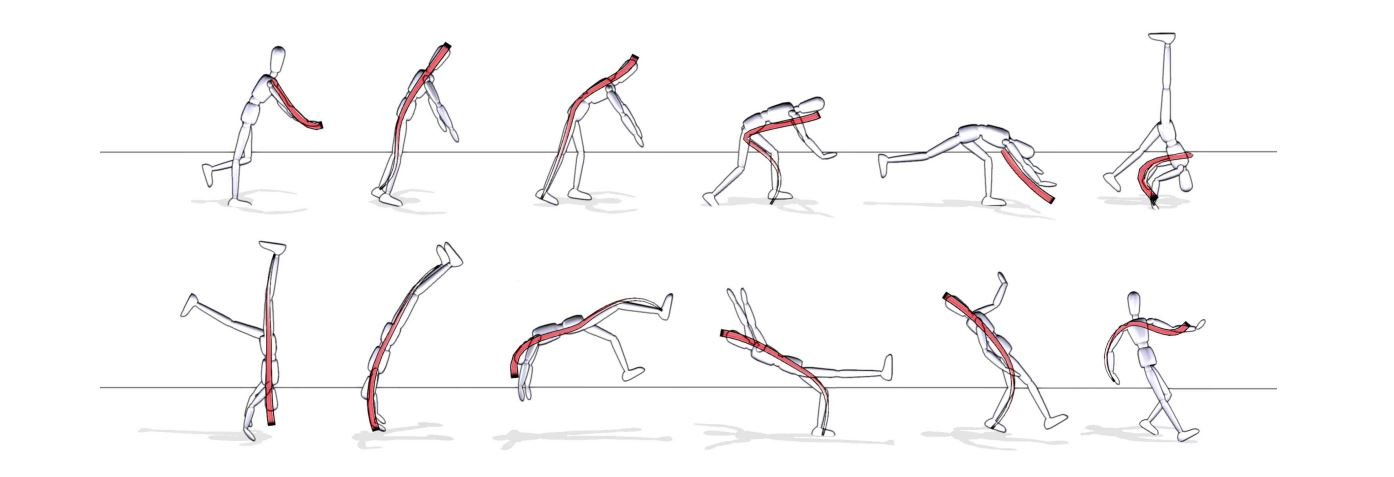
\includegraphics[scale=0.4]{img/baseline}
\caption{One character's keyframes using the line of action technique from \citep{guay2013line}.}
\end{figure}

The Line of Action: an Intuitive Interface for Expressive Character Posing -- 2013\\
Adding dynamics to sketch-based character animations -- 2015\\
Space-time sketching of character animation -- 2015\\
\\
Artist-oriented 3D character posing from 2D strokes -- 2016\\
people in Switzerland also did the posing \\
Sketch to pose in Pixar's presto animation system -- 2015


\section{Graph Theory}
Finding All the Elementary Cycles in a Directed Graph\\
A New Search Algorithm for Finding the Simple Cycles of a Finite Directed Graph\\
An Algorithm for Combining Graphs Based on Shared Knowledge

\section{Generating Animation}
%\subsection{cleaning/editing animation}
FootSee: an Interactive Animation System\\
Footskate Cleanup for Motion Capture Editing\\
SketchiMo: Sketch-based Motion Editing for Articulated Characters -- 2016\\
sketching for editing trajectories and poses

%\subsection{retargeting motion}
Retargetting Motion to New Characters\\
Using an Intermediate Skeleton and Inverse Kinematics for Motion Retargeting

%\subsection{generating animation}
Motion Graphs\\
Style-Based Inverse Kinematics -- 2004\\
generative models for motion capture sequences used to build animations\\\\
Displacement constraints for interactive modeling and animation of articulated structures -- 1994\\
fitting geometric constraints using physics\\\\
A constrained inverse kinematics technique for real-time motion capture animation -- 1999\\
Dancing-to-Music Character Animation

%\subsection{synthesis}
Synthesizing Dance Performance Using Musical and Motion Features -- 2006\\
between music and an animation generated from a motion graph built from motion capture

\chapter{Theoretical Foundations of Animation}

\section{Skeletons, Rigs, and Controllers}


\section{In-betweening}


\section{The Line of Action}


\section{Space-time Sketching}


\section{Optimization Problems}


\section{Rig Combinations as Trees}

\chapter{Implementing a Character Connection Algorithm}


\section{Interface}


\section{Intelligently Connecting Rigs}
Rather than changing the whole LOA concept and optimization algorithm, we reduce the more complex problem of using LOAs on multiple characters to the original LOA problem and utilize (nearly) the exact same minimization.

\section{Challenges}


\section{User Constraints}
Only allowed to connect and disconnect skeletons at keyframes.

\chapter{Experimental Validation of Solution}\label{results}

\section{Carefully Selecting Sample Keyframes}


\section{Establishing a Baseline for Comparison}


\section{Our Solution}

\subsection{Experiment}
Describe the performance metrics, experimental hypotheses, experimental conditions, test data,
and expected results. Provide the test data. Interpret the results of the experiments. Pay special
attention to cases where the experiments give no information or did not come out as expected.
Draw lessons and conclusions from the experiments. Explain how additional experiments could
validate or confirm results.

\subsection{Results}


\subsection{Conclusions and Future Experiments}

\chapter{Discussion}\label{chap:discussion}
Discussion lessons learned from the experiments, and new problems that are raised. 
\chapter{Conclusion}\label{chap:conclusion}
Give a summary of the problem, approach, implementation and evaluation. Discuss the principal
results in abstract terms. Discuss expected impact and further research directions.
Explain how the project satisfies the evaluation criteria for a Masters Research project. 
\appendix \chapter{Appendix}\label{chap:appendix}
\section{User Study Files}
Pose 1
\VerbatimInput{file/userpose1.txt}

Pose 2
\VerbatimInput{file/userpose2.txt}

Pose 3
\VerbatimInput{file/userpose3.txt}

\section{Links to Accompanying Videos}

\begin{itemize}
\item The Band Wagon Dancing in the Dark original scene - \url{https://www.youtube.com/watch?v=duLFwcsc6Nc}

\item The 10 main keyframes are annotated, along with inter-character contacts annotated by purple dots and ground contact annotated by blue dots - \url{https://www.youtube.com/watch?v=Xz3sYEbq_eo}

\item Densely annotated sub-clip using the \textit{previous} LOA method - \url{https://www.youtube.com/watch?v=02IyEHd3IfI}

\item Densely annotated sub-clip using the \textit{proposed} LOA method - \url{https://www.youtube.com/watch?v=q7cbzwNr7vY}

\item A side by side comparison of the two methods, with twists indicated in pink - \url{https://www.youtube.com/watch?v=TejQGyKDqwc}

\item Sped up 8x screen cast of the making of Pose 1 in Rumba - \url{https://www.youtube.com/watch?v=MCniYCZt9bg}

\item Sped up 8x screen cast of the making of Pose 2 in Rumba - \url{https://www.youtube.com/watch?v=058-576J4lM}

\item Sped up 8x screen cast of the making of Pose 3 in Rumba - \url{https://www.youtube.com/watch?v=EDtk6OqCbDE}

\item The baseline animation clip for future work - \url{https://www.youtube.com/watch?v=vdu0ETFJ95g}


\end{itemize}
%=========================================================


%=========================================================
\backmatter
\nocite{*}
\bibliographystyle{plain} % plain-fr si rapport en français 
\bibliography{bibfile}

%\cleardoublepage % Goes to an odd page
%\pagestyle{empty} % no page number
%~\newpage % goes to a new even page

\end{document}